\fullsys (\sys) is the abstraction of a group of batteryless intermittent sensors. \sys seeks to offer continuous sensing despite relying on ambient energy: an unpredictable and marginal power source. 
%orchestrates its nodes power cycles using a distributed approach (instead of relying on a master powerful node to coordinate coalesced nodes activities). 
%\sys seeks maximum time span of its underlying coalesced nodes through a distributed approach instead of a master node that orchestrates coalesced nodes on/off cycles. 

\subsection{Energy consumption}
%
\begin{figure}[t]
	\centering
		\begin{subfigure}{\columnwidth}
			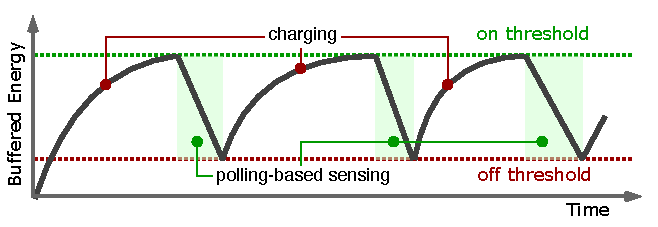
\includegraphics[width=\columnwidth]{figures/PowerCycleIntermittentSystem}
			\caption{When \sys does polling-based sensing, its energy consumption profile has, generally, two distinct levels.}
			\label{fig:pollingBasedSensing}
	\end{subfigure}
	\begin{subfigure}{\columnwidth}
		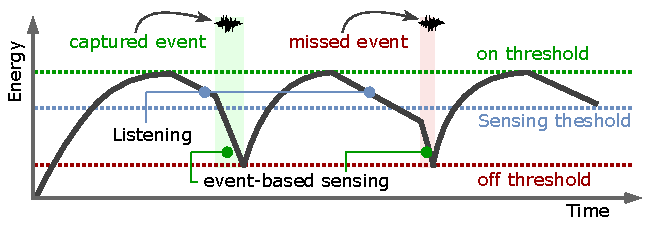
\includegraphics[width=\columnwidth]{figures/PowerCycleIntermittentSensor}
		\caption{When \sys does event-based sensing---staying in low power mode listening for an external event to happen---, its energy consumption profile has three distinct levels.}
		\label{fig:eventBasedSensing}
\end{subfigure}
		\caption{\fullsys energy profile for different sensing strategies}
		\label{fig:cisPwrCycle}
\end{figure} 
%
An intermittent sensor has a limited energy budget per power cycle. When it is tasked with a polling-based sensing activity, its energy consumption, generally, switches between two levels: zero when charging and a maximum when it activates its microcontroller  for data acquisition and processing, (see Figure~\ref{fig:pollingBasedSensing})---we assume that the microcontroller is the dominate energy consumer module of a node. However, in event-based sensing  a node puts its microcontroller into low power mode and waits (or listen) for an external event to wake up the microcontroller. This is important to minimize the energy wasted on the listening and to maintain the required energy budget for sensing for the longest possible time (Figure~\ref{fig:eventBasedSensing}). The idle listening mode, which is important for successful sensing, complicates the design of the \sys.

\subsection{On-time}
%
\begin{figure}[t]
		\centering
		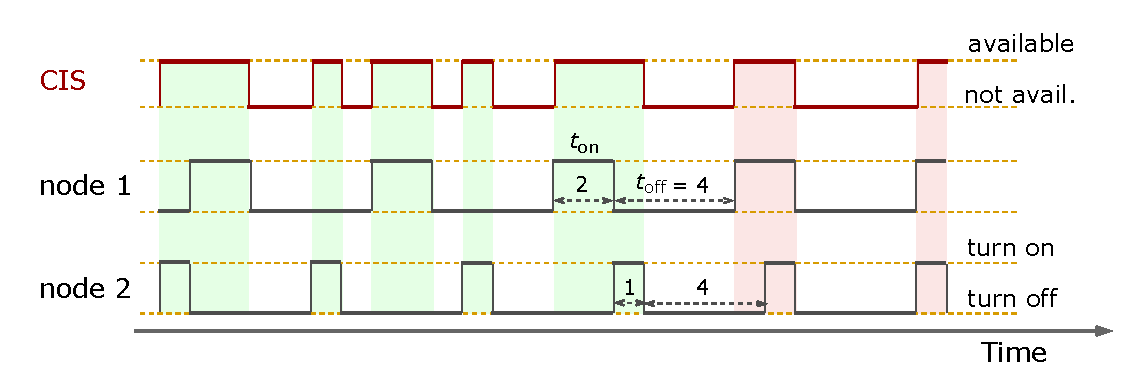
\includegraphics[width=\columnwidth]{figures/cisOntime}
		\caption{\fullsys's on-time is the projection of its intermittent nodes uptimes on the time axis. When the power cycles of the intermittent nodes are different their uptimes distribution approaches uniform distribution.}
		\label{fig:cisOntime}
\end{figure} 
%
The \sys's on-time is the projection of its underlying intermittent nodes' uptimes on the time axis. The \sys's on-time ranges from minimum (when all nodes cluster together, see the red regions in Figure~\ref{fig:cisOntime} to the maximum (when the overlapping between its nodes' uptimes is zero or when continuous time is reached). Two broad controlling strategies for approaching maximum \sys's time span can be imagined: 
\begin{enumerate}[wide, labelwidth=!, labelindent=0pt]
%
		\item \textit{Explicit on-time division method}: Recent advancements in intermittent timing enabled intermittent nodes to measure their on and off times (with help of an external ultra-low-power timer)~\cite{mayfly2017hester}. Passive light communication~\cite{marco} is mean for an ultra-low-power communication between batteryless nodes. Intermittent nodes can use these recent advancements to apply time division multiplexing strategy to explicitly avoid waking up at the same time slot. For example, a node calculates its average on-time $\overline{t_{on}}$ and off-time $\overline{t_{off}}$ for $N$ power cycles. Then it measures the time difference between its power-up and the intended transmitting time $\delta\tau$. Then it encodes the these information $({\overline{t_{off}}, \overline{t_{on}}, \delta\tau})$ in a message and broadcasts it. If a node receives this message it will have a full information about the transmitting node power cycle. It can then alter its power cycle, relative to the transmitting nodes cycle, by either increasing (or decreasing) its power consumption to shorten (or lengthen) its on-time and shift its power cycle. This approach, obviously, assumes relatively stable nodes power cycles. 
%
%\begin{figure}
%		\centering
%		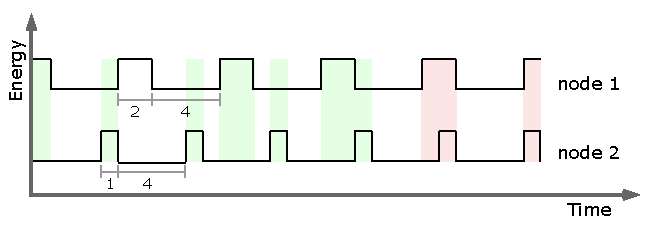
\includegraphics[width=\columnwidth]{figures/nodesDistribution}
%		\caption{When intermittent nodes power cycles are different their on-times tend to be uniformly distributed over the \sys power cycle}
%		\label{fig:implicitDistribution}
%\end{figure} 
%
		\item \textit{Implicit on-time division method}: With no information being exchanged between the intermittent nodes, the best \sys can do is to uniformly distribute its node's on-times and maintaining this distribution overtime. The key observation to enable uniform distribution of nodes' on-times is to ensure that their power cycles are different. Figure~\ref{cisOntime} shows the scenario of two intermittent nodes with a different power cycles. Node 1 has a power cycle of 6 units of time and an on/off cycle of $\frac{1}{3}$. Node 2 has a power cycle of 5 units of time and an on/off cycle of $\frac{1}{5}$. Following the time axis from the left, we can see that after the position of the on-time of Node 2 is shifted by 1 unit of time after each power cycle of Node 2. This implies that the on-time of Node 2 spends $\frac{1}{3}$ of the time clustered under the on-time of the Node 1 and the $\frac{2}{3}$ of the time while Node 1 is charging. When the intermittent nodes power cycles are uniformly distributed over the \sys power cycle, which equals the longest power cycle of its intermittent nodes, then the \sys on-time will evolve according to the following formula when a new node is added to the system
$$
	t_{on}(N) = t_{on}(N-1) + \frac{t_{off}(N-1)}{t_{off}(N-1)+t_{off}(N-1)} \times t_{on}(1),
$$
				where $t_{on}(N)$ is the on-time of a \sys with $N$ intermittent nodes.
\end{enumerate}
There is a clear trade-off between the aforementioned methods. While the explicit control method provide a fine control over the system distribution, the implicit method does not suffer from control messages exchange overhead. Although the implicit method is relatively simple to implement and explore, the explicit control method is not a far fetched idea considering the recent advancements in passive communication and intermittent timing. However, we opt to explore the implicit distribution control method as the hardware used to demonstrate the feasibility of passive light communication and ambient RF backscattering are not open source and re-making it is beyond the scope of this study.

\subsection{Power States}
From~\ref{fig:solarPwrCoIS} we can identify four operational stages for a \sys:
\begin{enumerate}
		\item \textit{Under-targeted energy conditions}---a \sys should be designed for near worst case energy conditions in order to comply with design requirements. However, a solar powered \sys, for example,  will come to a perpetual power down in the darkness. In general, for under-targeted energy conditions the system behavior is undefined.
		\item \textit{targeted energy conditions}---in these energy conditions the \sys should work intermittently and have sufficient randomness to distribute its intermittent nodes' power cycles to meet the desired availability percentage. 
\end{enumerate}


To meet a certain system availability, the system needs to be design for low energy conditions (i.e. artificial light).Depending on the ambient energy conditions, a \sys's power can vary significantly.  Generally, we can define four operational conditions that a \sys can experience.

\begin{figure}
		\centering
		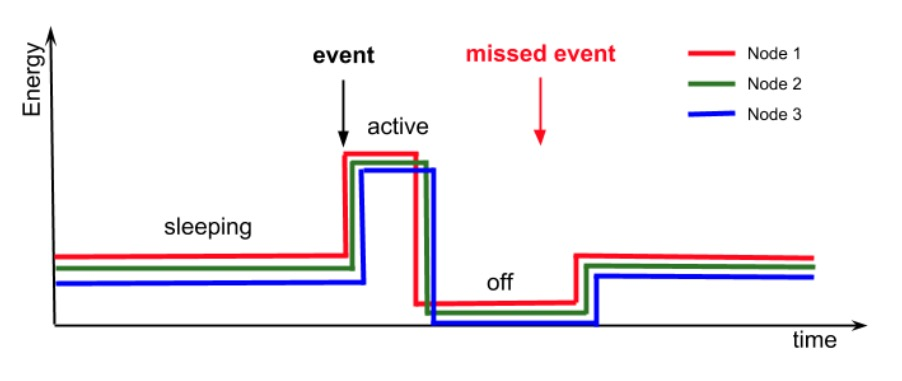
\includegraphics[width=\columnwidth]{figures/noRandomization}
		\caption{\todo{Placeholder} No randomization}
		\label{fig:noRand}
\end{figure} 

\begin{figure}
		\centering
		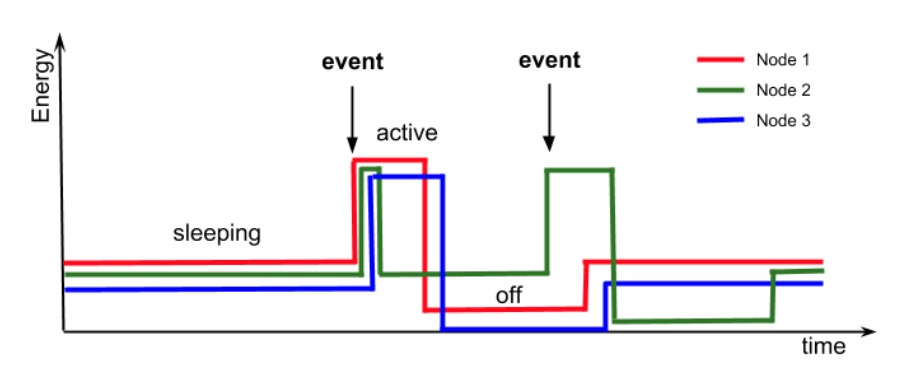
\includegraphics[width=\columnwidth]{figures/randomization}
		\caption{\todo{Placeholder} Randomization}
		\label{fig:noRand}
\end{figure} 

\begin{figure}
		\centering
		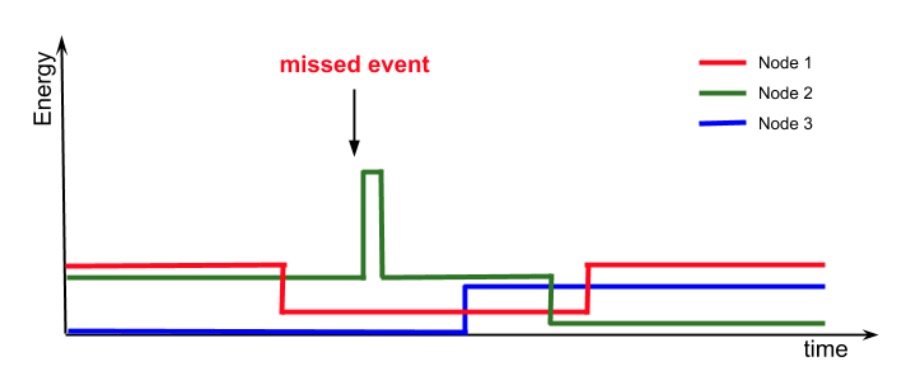
\includegraphics[width=\columnwidth]{figures/randomizationSideEffect}
		\caption{\todo{Placeholder} Randomization side effect}
		\label{fig:noRand}
\end{figure} 


